\documentclass[11pt]{article}
\usepackage[margin=1in]{geometry}
\usepackage{amsmath}
\usepackage{booktabs}
\usepackage{graphicx}
\usepackage{tabularx}
\usepackage{caption}
\usepackage{microtype}
\usepackage{url}
\usepackage[hidelinks]{hyperref}
\urlstyle{tt}
\newcommand{\modelonly}{\textsc{model-only}}
\newcommand{\code}[1]{\texttt{\small #1}}

\title{\textbf{Resilient Emergency MANETs for Wilderness Safety}\\[4pt]
\large Supplementary Materials: Artifact Guide, Reproduction Instructions,
and Extended Results}
\author{Ethan Doherty\\\small Directed Study (CS 5976) --- Advisor: Prof.~Guevara}
\date{July 26, 2026}

\begin{document}
\maketitle

\noindent This supplement accompanies
\emph{Resilient Emergency MANETs for Wilderness Safety: Directed Study Final
Report} (2026-07-26). Section~\ref{s:artifacts} maps every artifact the report
cites to its location in the project repository
(\code{github.com/edoherty2017/resilient-emergency-manets}, branch
\code{trial2-field-campaign-2026-07} --- the canonical version of all
material). Section~\ref{s:running} gives verified commands for running the
simulator. Sections~\ref{s:figures}--\ref{s:table} present extended views of
the released year-scale results. All simulation values are \modelonly{}
(uncalibrated), drawn exclusively from the released
\code{release\_v1} aggregates.

\section{Guide to the artifact repository}\label{s:artifacts}

\begin{table}[h]
\small
\begin{tabularx}{\textwidth}{@{}p{5.6cm}X@{}}
\toprule
\textbf{Report section} & \textbf{Repository location} \\
\midrule
\S5.2--5.3 year-scale results & \path{artifacts/sim/corrected/release_v1/} (\code{corrected\_stats.json}, \code{meaningful\_metrics.json}; locked inputs and hashes alongside) \\
\S4 parity, reproducibility, tests & \path{artifacts/sim/corrected/} (\code{micro\_parity\_2026-07-17.json}, \code{repro\_check\_2026-07-17/}, \code{cargo\_test\_2026-07-26.log}) \\
\S5.1 Trial 1 and ITM screens & \path{artifacts/airmap/live_trial/quality_gates.json}; \path{artifacts/coverage_prediction/}; \path{artifacts/itm/} \\
\S6 Trial 2 registrations & \path{artifacts/trial2/} (prediction packs, \code{prereg\_manifest.json}) and the dated siting documents in \path{docs/} \\
\S6 field raw evidence & \path{artifacts/trial2/raw_pull_20260721/}, \path{raw_pull_20260726/} (SHA-256 checksums within) \\
\S6.6 station-cadence evidence & \path{artifacts/trial2/nhmesh_activity_20260726/} \\
Raw dataset release & \path{artifacts/dataset_release/evidence-2026-07-26/} \\
\bottomrule
\end{tabularx}
\caption{Report citations to repository paths. Registrations are
git-timestamped by commit \code{1229309}; every SHA-256 digest cited in the
report re-verifies with \code{shasum -a 256}.}
\end{table}

The 2026-07-17 report draft and the \path{WITHDRAWN-DO-NOT-CITE/} directory
are retained archives only; project claims should not be reviewed from them.

\section{Running the simulator}\label{s:running}

Requirements: a Rust toolchain (\code{rustup}) for the release engine;
Python~3.12+ with the repository virtual environment for the reference engine
and analysis scripts. All commands run from the repository root and were
executed successfully on 2026-07-27.

\paragraph{Build.}
\begin{verbatim}
(cd fastsim && cargo build --release)
\end{verbatim}

\paragraph{Single run.} One simulated day completes in roughly two seconds; a
full 365-day statewide year in about 3.5 minutes:
\begin{verbatim}
./fastsim/target/release/fastsim \
  --topology artifacts/sim/topology_statewide.json \
  --routes   artifacts/sim/routes_statewide.json \
  --weather  artifacts/sim/weather_year.json \
  --config   config/sim/wmnf_sim.yaml \
  --mode duty_sync --days 365 --seed 42 --out /tmp/year.json
\end{verbatim}
The \code{--mode} argument accepts: \code{flood}, \code{min\_hop},
\code{etx}, \code{energy\_aware}, \code{lb\_energy}, \code{duty\_sync},
\code{duty\_adaptive}, \code{rotate\_lb}, \code{selective\_duty}.

\paragraph{Reproduce the released sweep.} Nine modes $\times$ seeds 42--46
with hash-locked inputs and an aggregate manifest:
\begin{verbatim}
scripts/run_corrected_release.sh /tmp/my_release
\end{verbatim}
Compare \code{/tmp/my\_release/corrected\_stats.json} against
\path{artifacts/sim/corrected/release_v1/corrected_stats.json}.

\paragraph{Verification suite.}
\begin{verbatim}
(cd fastsim && cargo test)                    # 47 + 3 tests
.venv/bin/python scripts/sim_micro_parity.py  # cross-engine parity
\end{verbatim}

\section{Extended results figures}\label{s:figures}

\begin{figure}[h]
\centering
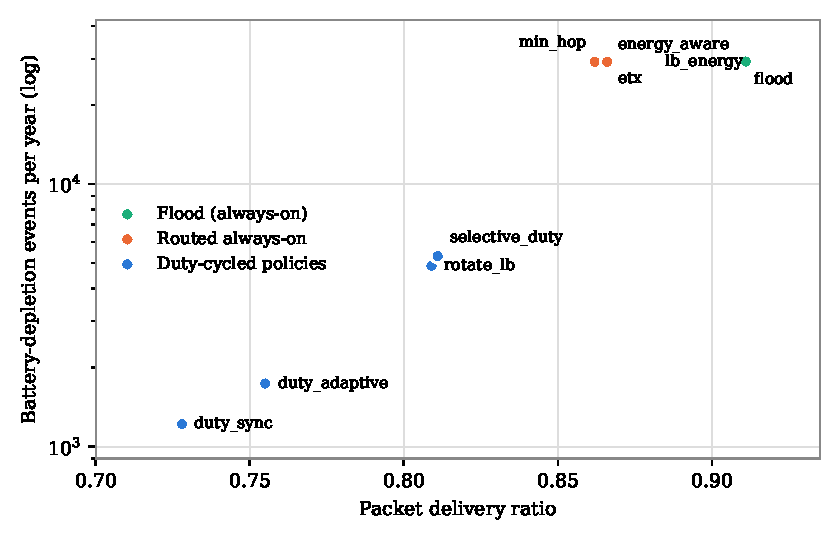
\includegraphics[width=0.82\textwidth]{figures/fig_s1_tradeoff_scatter.pdf}
\caption{The survivability trade (\modelonly, uncalibrated; release\_v1,
five-seed means, PDR CIs $< \pm 0.003$). The five always-on routing modes
cluster indistinguishably at 29{,}164--29{,}234 depletions per year across a
0.05 span of delivery ratio; duty-cycled policies occupy a separate regime,
5.5--24$\times$ fewer depletions at 0.05--0.14 lower delivery ratio. No
overall winner is declared; the frontier is the finding.}
\end{figure}

\begin{figure}[h]
\centering
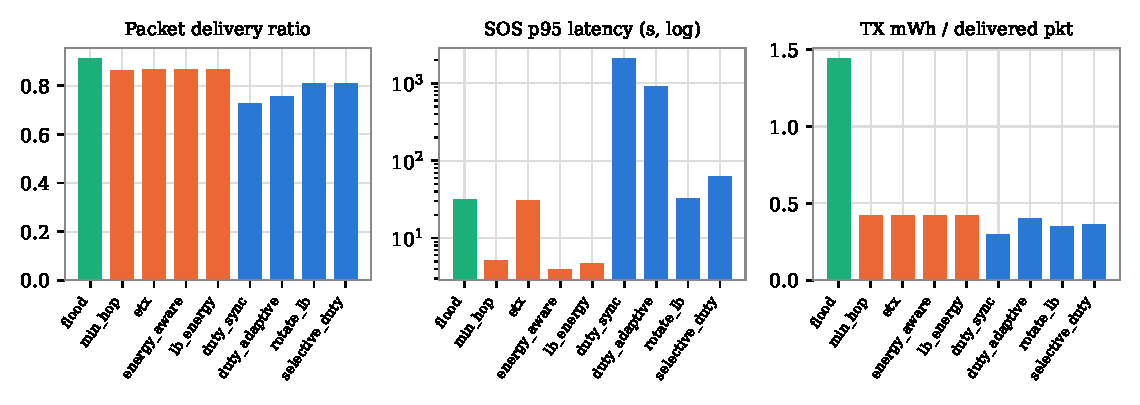
\includegraphics[width=\textwidth]{figures/fig_s2_cost_panels.pdf}
\caption{The cost side of duty-cycling (\modelonly): delivery ratio, SOS
95th-percentile latency (log scale; duty\_sync's 94.7\% delivery conceals a
35-minute p95 while backbone-awake duty modes hold 33--62\,s), and transmit
energy per delivered packet.}
\end{figure}

\clearpage
\section{Full results table}\label{s:table}

\begin{table}[h]
\centering\small
\setlength{\tabcolsep}{4pt}
\begin{tabular}{@{}lcccccccc@{}}
\toprule
Mode & PDR & $\pm$CI & Deaths/yr & $\pm$CI & SOS del. & SOS p95 & Avail. & mWh/pkt \\
\midrule
flood          & 0.911 & 0.0001 & 29{,}234 & 1.4 & 100\%  & 32\,s     & 53.5\% & 1.44 \\
min\_hop       & 0.862 & 0.0002 & 29{,}164 & 1.4 & 100\%  & 5\,s      & 53.7\% & 0.42 \\
etx            & 0.866 & 0.0002 & 29{,}165 & 2.0 & 100\%  & 31\,s     & 53.7\% & 0.42 \\
energy\_aware  & 0.866 & 0.0002 & 29{,}164 & 2.1 & 100\%  & 4\,s      & 53.7\% & 0.42 \\
lb\_energy     & 0.866 & 0.0002 & 29{,}164 & 1.4 & 99.9\% & 5\,s      & 53.7\% & 0.42 \\
duty\_sync     & 0.728 & 0.0002 & 1{,}217  & 1.1 & 94.7\% & 35.0\,min & 96.5\% & 0.30 \\
duty\_adaptive & 0.755 & 0.0028 & 1{,}737  & 0.9 & 99.3\% & 15.0\,min & 94.7\% & 0.40 \\
rotate\_lb     & 0.809 & 0.0002 & 4{,}877  & 2.3 & 99.5\% & 33\,s     & 91.0\% & 0.35 \\
selective\_duty& 0.811 & 0.0001 & 5{,}311  & 5.3 & 99.3\% & 62\,s     & 89.7\% & 0.36 \\
\bottomrule
\end{tabular}
\caption{Complete release\_v1 results (\modelonly, uncalibrated): nine modes
$\times$ seeds 42--46 $\times$ 365 days; means with t-based 95\% confidence
half-widths. Source: \code{corrected\_stats.json},
\code{meaningful\_metrics.json}.}
\end{table}

\end{document}
